
\documentclass[t, 11pt]{beamer}
%\pdfmapfile{+sansmathaccent.map}
%%% Работа с русским языком
\usepackage{cmap}				
\usepackage{mathtext} 				
\usepackage[T2A]{fontenc}		
\usepackage[utf8]{inputenc}			
\usepackage[russian, english]{babel}	

\usetheme{Montpellier}
\usecolortheme{beaver} % Цветовая схема



%%% Работа с картинками
\usepackage{graphicx}

\usepackage{csquotes}

\hypersetup{				
	colorlinks=true,       	
	linkcolor=blue,          
	citecolor=black,       
	filecolor=magenta,      
	urlcolor=red           
}
%% табличка
\usepackage{booktabs, caption, makecell}
\usepackage{threeparttable}

%% график нормального распределения 
\usepackage{tikz}
\usepackage{xcolor}
\usepackage{pgfplots}
\pgfplotsset{compat=1.7}

%% доп символы
\usepackage{newunicodechar}

\newcommand\Warning{%
	\makebox[1.4em][c]{%
		\makebox[0pt][c]{\raisebox{.1em}{\small!}}%
		\makebox[0pt][c]{\color{red}\Large$\bigtriangleup$}}}%

%\newunicodechar{⚠}{\Warning}

\title {Statistical tests}
\subtitle{Intro to Statistical Inference Part 1}
\author{Chuvakin Sergey}
\date{\today}
\institute[<<Anthropology>>]{<<School of Advanced Studies>>}

\begin{document}

	
	\frame[plain]{\titlepage}		
	
	\section{Outline}
	
		\begin{frame} 
			\frametitle{\insertsection} 
			\begin{itemize}
				\item Why do we need it?
				\item Statistical inference (what about sample?)
				\item Hypothesis 
				\item Type of errors
				\item Box-plot explanation
				\item Compare two means 
				\item T-test
				\item Degrees of freedom
				\item Dependent and Independent samples
				\item Variance check
				\item Normallity check 
				
			\end{itemize}
\end{frame}
	
	\section{Why do we need it?}
	
	\begin{frame}
		\frametitle{\insertsection} 
		\framesubtitle{\insertsubsection} 
		Suppose you have a question (aka research question). 
		
		There are tons of way to answer it. 
		
		\vspace{1cm}
		
		\Warning But - how to do it scientifically?
		
	\end{frame}		

	\section{Statistical inference}

	\begin{frame}
		\frametitle{\insertsection} 
		\framesubtitle{\insertsubsection} 
	
		Statistical Inference - is a way to answer question using a data. 
		
		Statistical inference - is a core of Data Driven Approuch in a business. 
		
		\vspace{1cm}
		
		\Warning Helps to establish the fact of \emph{significance} of \textbf{change} of some variable or \textbf{difference} between some variables (colud also be a relation between varaibles). Main goal is to expand inference from Sample to Population
		\vspace{1cm}
		
		\textbf{Example}: How people waste their money on insurance?
		%  Does men waste more money on insurance than women?
		
	\end{frame}		

	
	\section{Hypothesis} 
	\begin{frame}
		\frametitle{\insertsection} 
		\framesubtitle{\insertsubsection} 
		
		
			Hypothesis - formal way to state a scientific question. Could and should be tested! 			
			
			\vspace{1cm}
			
			\Warning Research Question $\neq$ Hypothesis 
			
			\vspace{1cm}
			
			Typically, a statistical hypothesis is the statement about (a) the relationship between two variables or (b) the characteristics of a distribution of a variable.
			
	
	\end{frame}		

	\begin{frame}
	\frametitle{\insertsection} 
	\framesubtitle{\insertsubsection} 
	
 		All hypothesis contain two parts - \textbf{Alternative} Hypothesis and \textbf{Null} Hypothesis 
 		
 	\vspace{1cm}
 	
 	\begin{itemize}
 		\item Substantive hypothesis (a.k.a. alternative; H1) is the research hypothesis, that is (typically), the statement that there is some relation between the phenomena under investigation
 		 \item Null hypothesis (H0) is the statement that there is no relation between the phenomena under investigation. Simply speaking, H0 states that H1 is false.
	\end{itemize}
	
	\end{frame}		


    \subsection{Example}
    
    	\begin{frame}
    	\frametitle{\insertsection} 
    	\framesubtitle{\insertsubsection} 
    	\textbf{Research Question}: How people waste their money on insurance?
    	
    	\textbf{H1}: Men tend to waste more money on insurance 
    	
    	\textbf{H0}: There is no differences between men' s and women behavior 
    	
    	\textbf{H1}: People in southwest region tend to spend more momey on insurance
    	
    	\textbf{H0}: There is no differences between people in different regions 
    	
    \end{frame}		

    \subsection{Important!}


    	\begin{frame}
	\frametitle{\insertsection} 
	\framesubtitle{\insertsubsection} 
	
	
	\Warning  \textbf{Neither H1 nor H0 can be true or false}. Hypothesis can only be rejected. 
	
	\vspace{1cm}
	
	\begin{enumerate}
     	\item \textbf{True} means that a hypothesis can not be reasonably rejected given the observed data 
		\item \textbf{False} means that a hypothesis can be reasonably rejected given the observed data
	\end{enumerate}
	
	\vspace{1cm}
	
		\textbf{NB}: If H0 is rejected by the data, one can accept H1. However, if H1 is rejected by the data, it does not mean that one can accept H0
		
	\end{frame}		

	\section{Type of errors}
    	\begin{frame}
	\frametitle{\insertsection} 
	\framesubtitle{\insertsubsection} 
	
	\begin{center}
		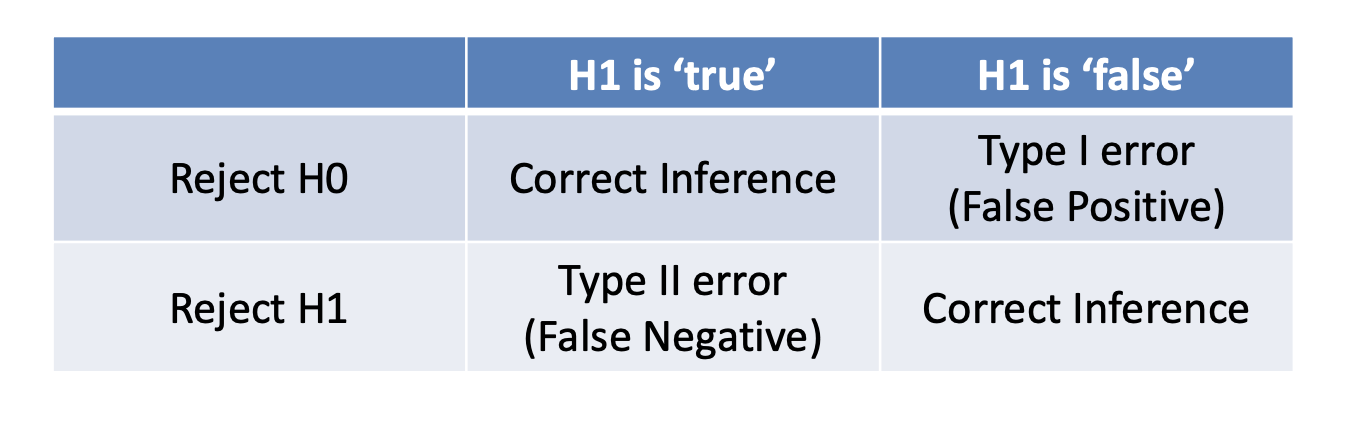
\includegraphics[scale=0.5]{er1}
	\end{center}
\end{frame}	

    	\begin{frame}
	\frametitle{\insertsection} 
	\framesubtitle{\insertsubsection} 
	
	\begin{center}
		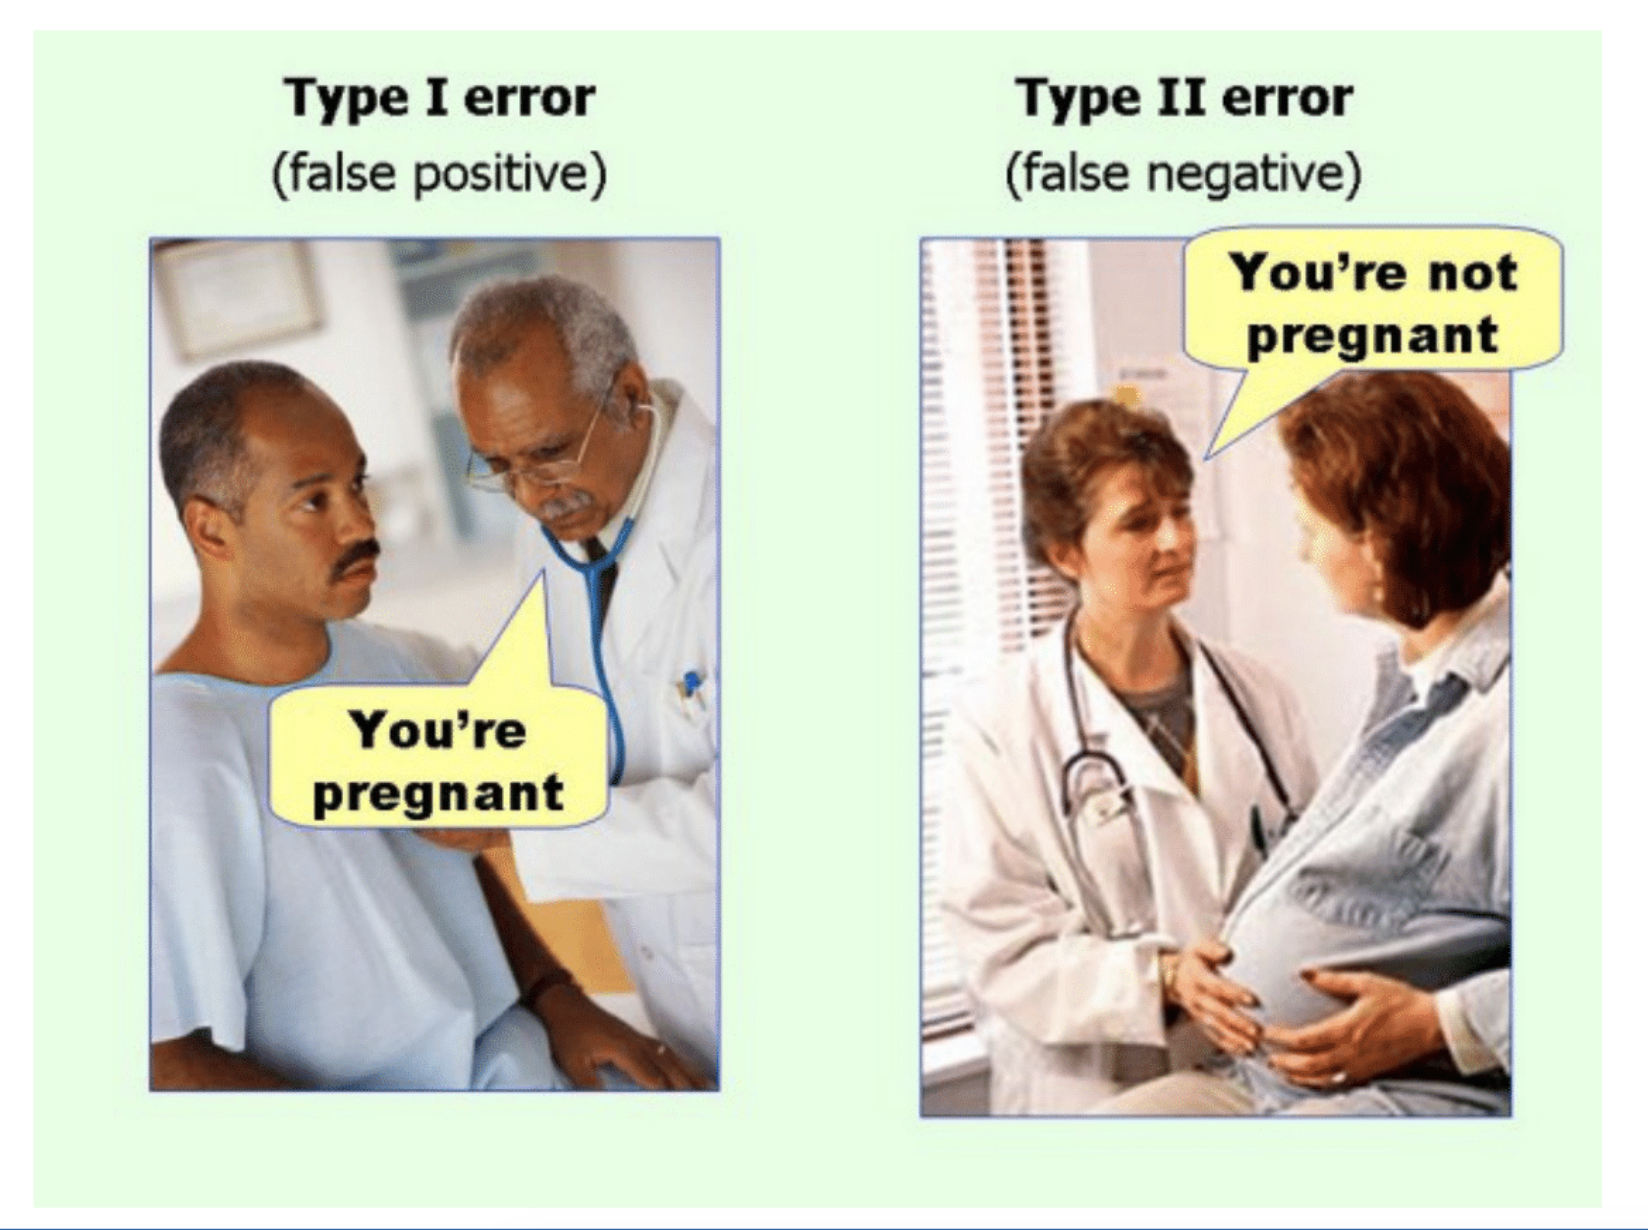
\includegraphics[scale=0.3]{er2}
	\end{center}
\end{frame}	

\section{Compare two means }
\subsection{Box-plot explanation}

    	\begin{frame}
	\frametitle{\insertsection} 
\framesubtitle{\insertsubsection} 
	\begin{center}
		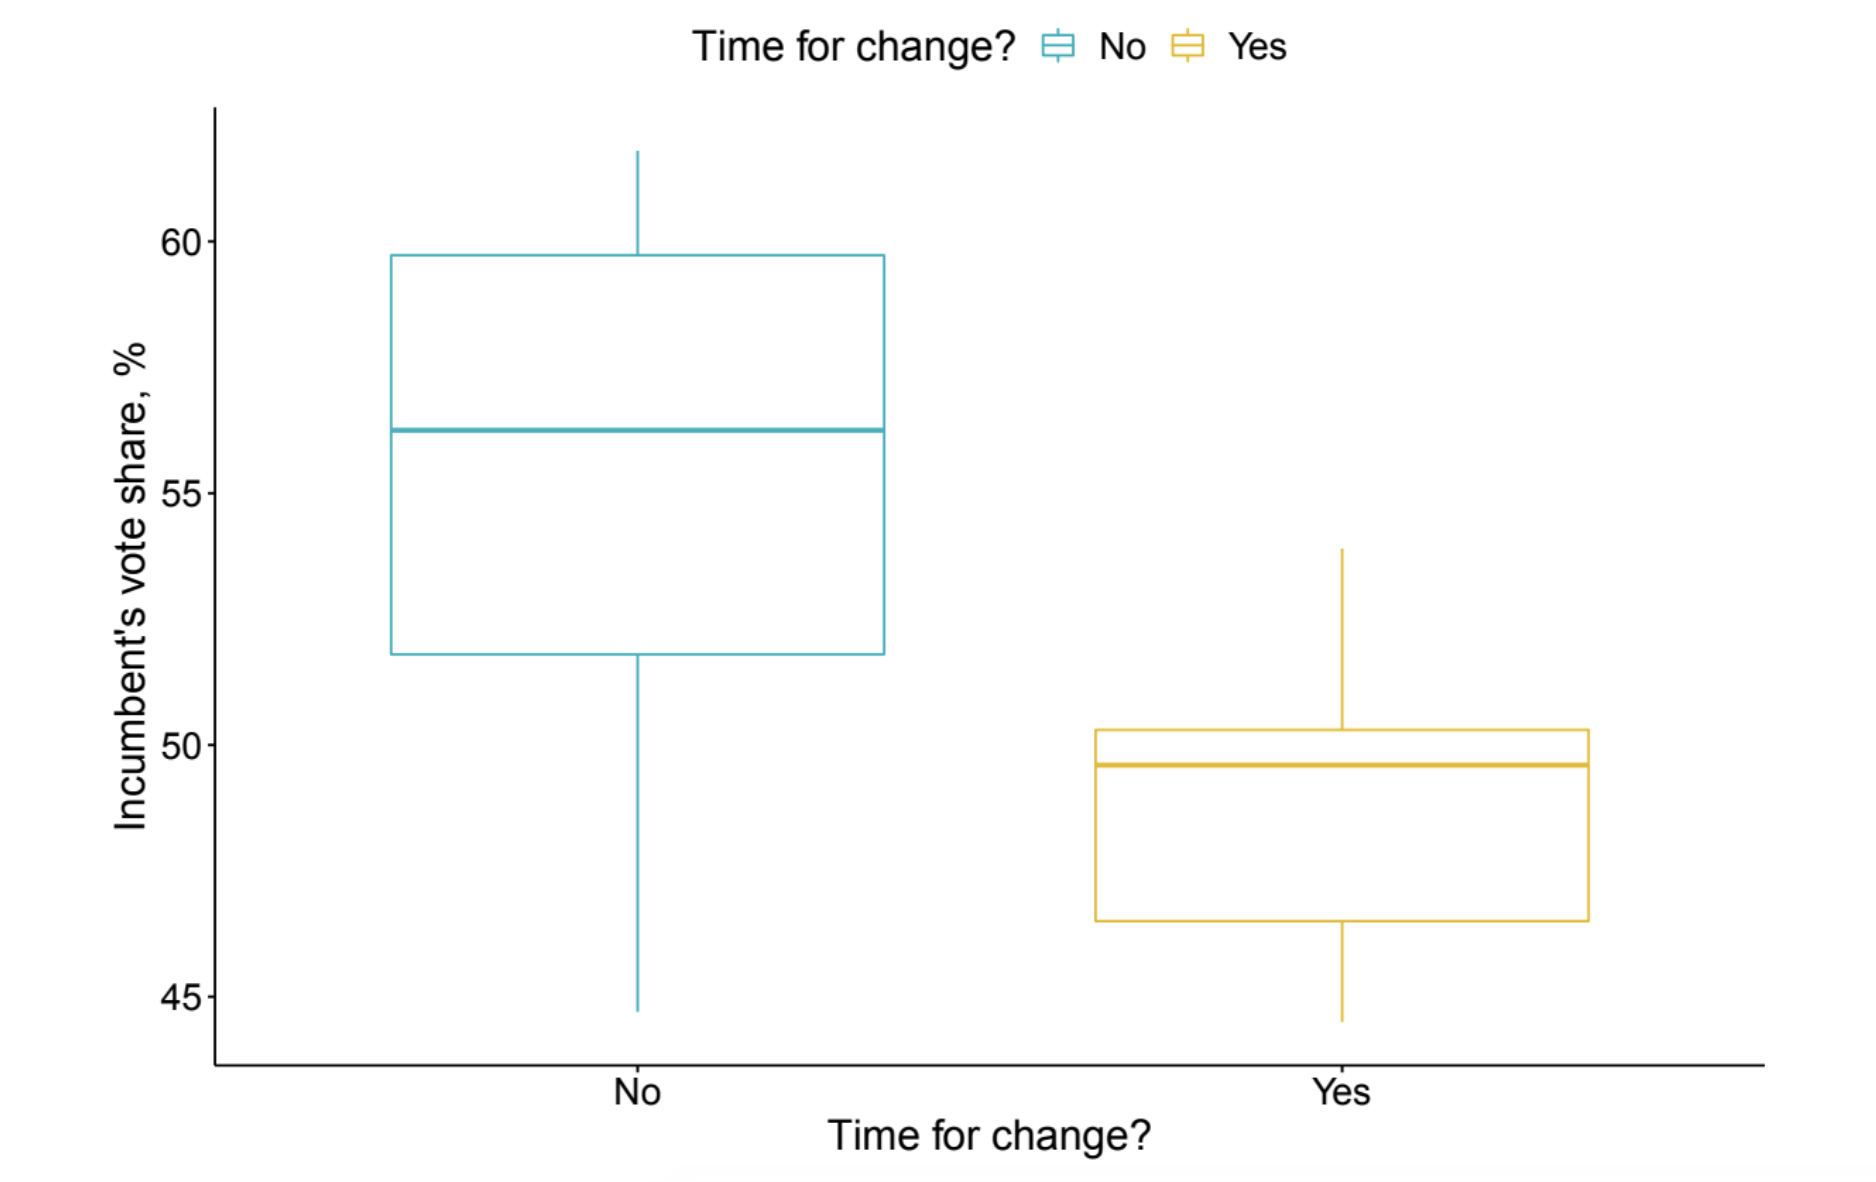
\includegraphics[scale=0.3]{boxp1}
	\end{center}

	\end{frame}	

    	\begin{frame}
	\frametitle{\insertsection} 
	\framesubtitle{\insertsubsection} 
	\begin{center}
		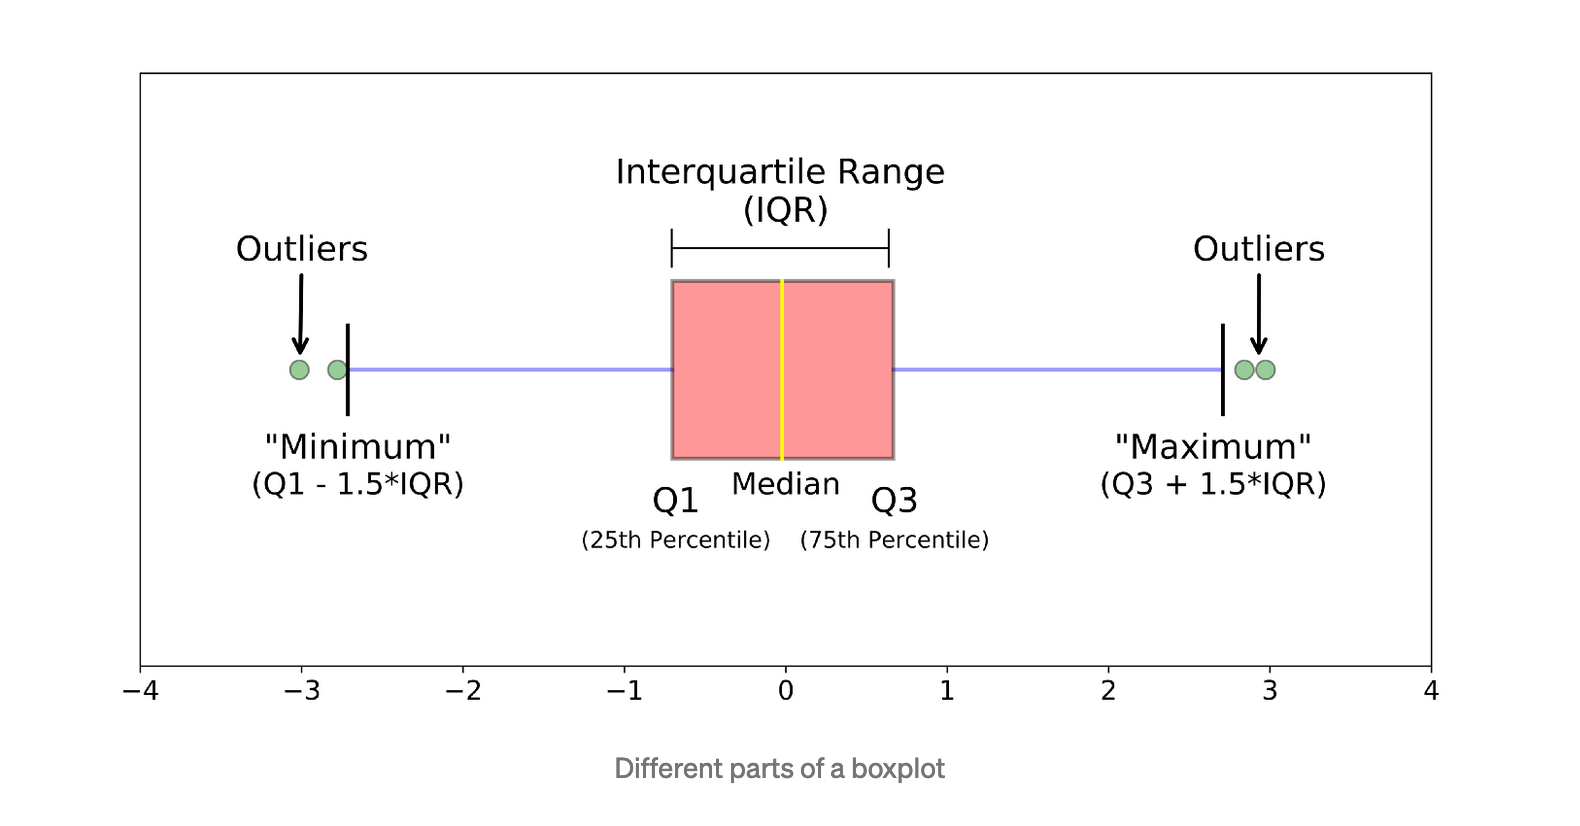
\includegraphics[scale=0.4]{boxp2}
	\end{center}
	
\end{frame}	

\subsection{What is an outlier?}
    	\begin{frame}
	\frametitle{\insertsection} 
	\framesubtitle{\insertsubsection} 
	
	Outlier - is an extra observation(s) that extremely differs from other in one variable.
	
	\vspace{1cm}
	
	Rule of $1.5 \times IQR$
	
	\vspace{1cm}
	
	Follow \href{https://www.khanacademy.org/math/statistics-probability/summarizing-quantitative-data/box-whisker-plots/a/identifying-outliers-iqr-rule}{here} tutorial
\end{frame}	


\subsection{T-test}
\begin{frame}
	\frametitle{\insertsection} 
	\framesubtitle{\insertsubsection} 
	
	Back to our first H1 - Men tend to waste more money on insurance?
	
	\begin{center}
		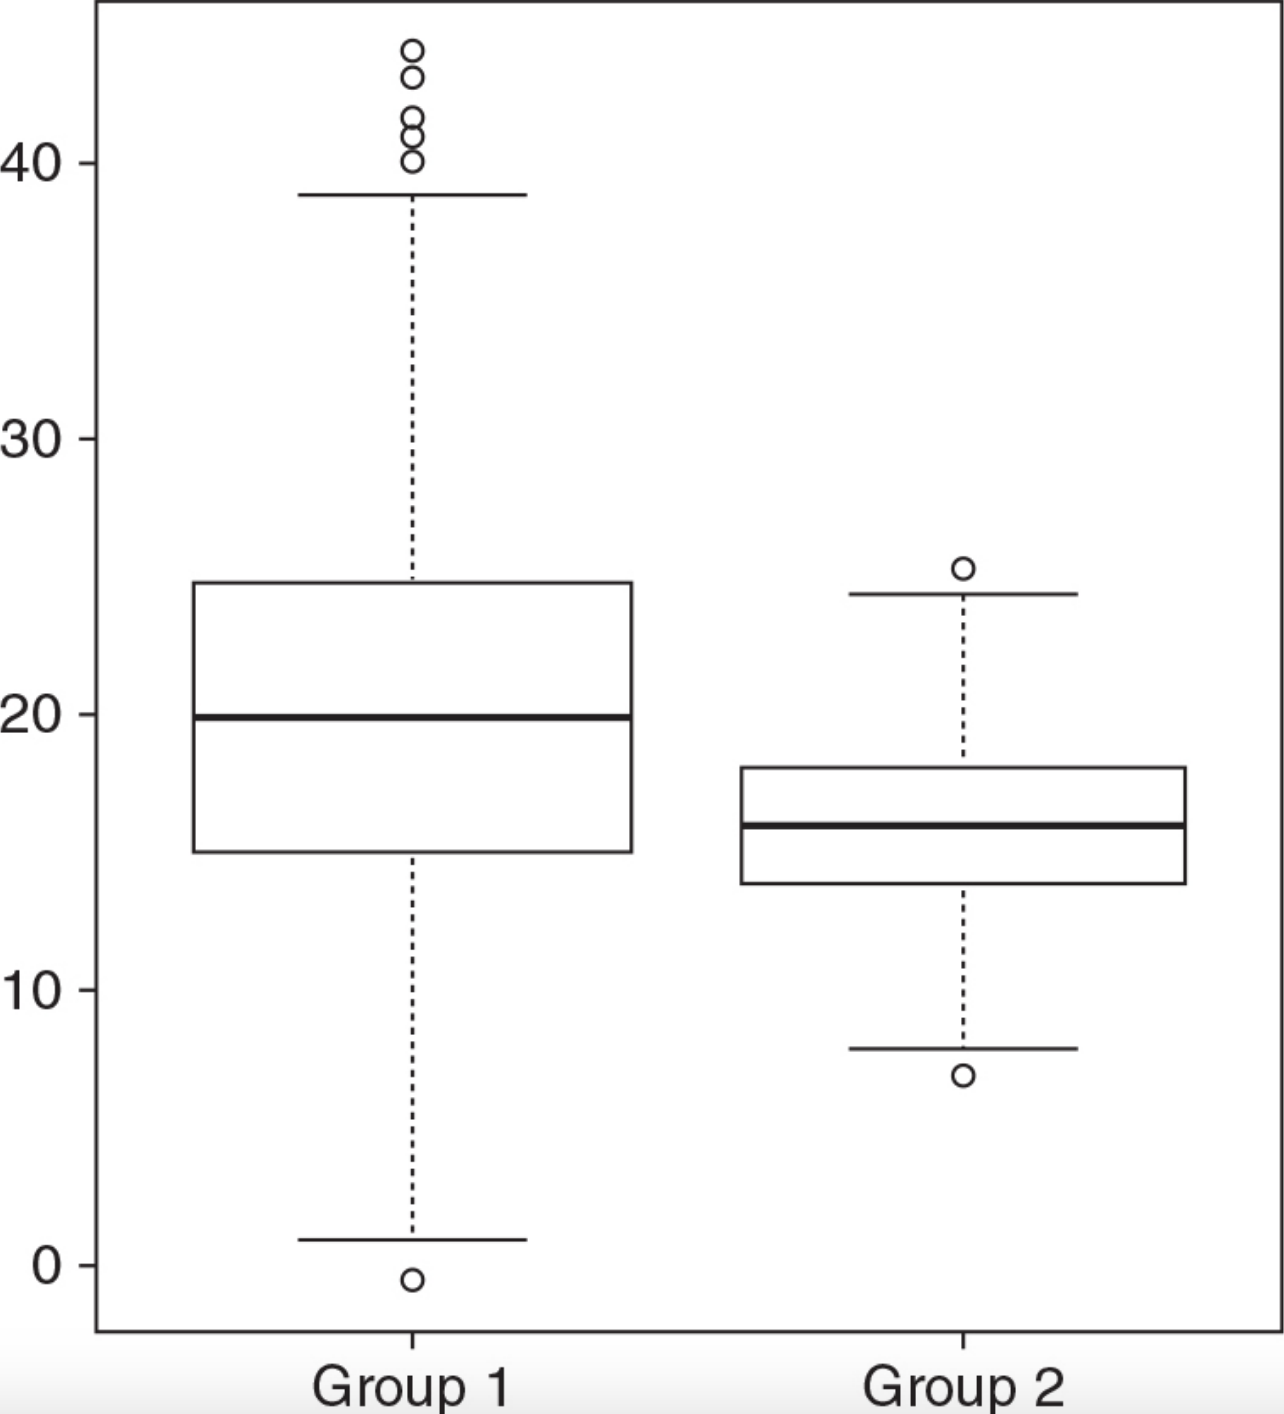
\includegraphics[scale=0.17]{boxp3}
	\end{center}

 Say it is real data - what can you say here?
	 
\end{frame}	
    
    \begin{frame}
    	\frametitle{\insertsection} 
    	\framesubtitle{\insertsubsection} 
    	Answer - almost nothing. The only way state the difference is to conduct statistical test. 
    	
    	\vspace{1cm}
    	
    	T-test - statistical technic to answer the question, wheather two groups are different on some variable. 
    	
    	\vspace{0.5cm}
    	
    	Anyway - you can notice that group different, but formal test suggest whether it \emph{significant!}
    	
    	\vspace{0.5cm}
    	
    	\textbf{Significance} - statistical feature which states that with growing number of observation difference persists. 
    	
    \end{frame}	


    \begin{frame}
	\frametitle{\insertsection} 
	\framesubtitle{\insertsubsection} 
	
	
	Formally:
	
	\begin{itemize}
	
    
    \item Null hypothesis (H0): $\mu_1 =\mu_2  $
	
	\item Alternative hypothesis (H1): $\mu_1 \neq \mu_2 $
	
	\item Test statistic is given by:
	
	$$t = \frac{\hat{\mu_1} -\hat{\mu_2} }{\sqrt{ \frac{\hat{\sigma_1^2}}{n_1}  -  \frac{\hat{\sigma_2^2}}{n_2 }}}$$
	
	
	where $\mu_1$ and $\mu_2$ are sample (estimated) means, $\sigma_1^2$ and $\sigma_2^2$are sample (estimated) variances, and n1 and n2 are sample sizes for Groups 1 and 2.
	 
  \item In t-test, there are two basic summaries of the data: test statistics and degrees of freedom
	\end{itemize}
\end{frame}	

\subsection{Afterwards}
	
	\begin{frame}
		
		\frametitle{\insertsection} 
		\framesubtitle{\insertsubsection} 
		
		\begin{itemize}
			\item Count Degrees of freedom
			\item Count T-test
			\item Choose Confidence level
			\item Look at \href{https://www.sjsu.edu/faculty/gerstman/StatPrimer/t-table.pdf}{this matrix}
			\item Make inference
		\end{itemize}
		
		
		\end{frame}	
	    

	\subsection{Thats all?}
	
	\begin{frame}
		
		\frametitle{\insertsection} 
		\framesubtitle{\insertsubsection} 
		
		Not yet. 
		
		\begin{itemize}
			\item How to find Degrees of freedom?
			\item Are groups independent?
			\item Are variances equal?
			\item Does target varaible normally distributed?
		\end{itemize}
		
		
	\end{frame}	

\subsection{Degrees of freedom}

	\begin{frame}
		\frametitle{\insertsection} 
		\framesubtitle{\insertsubsection} 
		Degrees of freedom (df) is a kind of measure of model complexity.
		
		\vspace{1cm}
	
		\begin{itemize}		
		\item Formally speaking, it is the number of values in the finalcalculation of a statistic that are free to vary.
		
		\item 	If you are a manager of a football team, you can freely determine positions of 9 out of 10 field players (if you choose sequentially).
		
		\item 	To put it simply,df is the difference between the number of observations (independent information peaces) you have and the number of parameters you use to estimates some test statistic of interest:
			$$df=n_o - n_p$$
		
	\end{itemize}

	\end{frame}	

	\begin{frame}
	\frametitle{\insertsection} 
	\framesubtitle{\insertsubsection} 
	
	The defailt df formula is given by the Welch–Satterthwaite equation:
\[
df=\frac{\frac{s_{1}^{2}}{n_1}+\frac{s_{2}^{2}}{n_2}}{\frac{\frac{s_{1}^{2}}{n_1}}{n_1-1}+\frac{\frac{s_{2}^{2}}{n_2}}{n_2-1}}
\]
Basic intuition: $df  = n_{row} - n_{col}$ 
\end{frame}	

\subsection{Target varaible distribution}
	\begin{frame}
	\frametitle{\insertsection} 
	\framesubtitle{\insertsubsection} 
	
	It should be continious, and at least peudo normally distributed. You can check it in two ways:
	
	Numerical:
		\begin{itemize}
		\item Shapiro-Wilk test. Null hypothesis: no large deviations fromthe normal distribution. If shapiro.test()results in large (i.e. insignificant) p-values, we cannot reasonably reject the null so we may safely assume that normality holds: This is theoretically incorrect (we actually test H1 of non-normality) but still the standard practice.
		\item  Kolmogorov-Smirnov (K-S) normality test. 
		\end{itemize}
	\end{frame}
	\begin{frame}
	\frametitle{\insertsection} 
	\framesubtitle{\insertsubsection} 
	Graphical:
	\begin{itemize}
		\item density plots/histograms: is the empirical density of Y close to the bell-shape curve? Not very useful with extremely small samples.
		\item QQ-plots (QQ forquantile-quantile): does individual observations are close enough to the 45-degree line?
	\end{itemize}

	
	\end{frame}	

	 \subsection{Homogeneity of variances}
	
	\begin{frame}
		\frametitle{\insertsection} 
		\framesubtitle{\insertsubsection} 
		
	Homogeneity of variance means that we assume that two populations under comparison (from which we sample comparison groups) may differ in their means but not variances.
	
	\vspace{1cm}
	
	We can check variances using F-test. In R - var.test(). Alternatives bartlett.test(), leveneTest() (car package), fligner.test()
	
	\end{frame}	

	 \subsection{Dependents Samples}

	\begin{frame}
		\frametitle{\insertsection} 
		\framesubtitle{\insertsubsection} 
		\begin{itemize}
		\item The standard t-test assumes that different individuals are randomly assigned to one of two conditions, so their Y scores are independent (i.e a score of ani-th individual is not influenced by a score of an i-th individual: no spillover effects)
		
		\item Dependent (paired) samples:
		\begin{itemize}
		\item	Same individuals sequentially exposed to two different conditions
		
		\item There are many pairs consisting of two very similar (identical or matched) individuals. In each pair, one individual is(randomly) assigned to one condition and the other assigned to another condition (e.g., experiments with twins).
	\end{itemize}
	\end{itemize}
		
	\end{frame}	

	\begin{frame}
	\frametitle{\insertsection} 
	\framesubtitle{\insertsubsection} 
		
		Test statistic is computed in a different way:
		
		$$t = \frac{\hat{D} - \mu_0}{  \frac{\sigma_D}{  \sqrt{n_D}  }    }$$
		
		where D is the sample average within-pair difference,$\mu_0$ is some constant (typically 0, because the default $H_0$: D = 0; read about one-sample t-test for details),$\sigma_D$i s the estimatedstandard deviation of within pair differences, and $n_D$ is thenumber of pairs
		
		\vspace{1cm}
		
	R implementation: set the paired argument of t.test() to True
\end{frame}	


	\subsection{what can be done}
	\begin{frame}
	\frametitle{\insertsection} 
	\framesubtitle{\insertsubsection} 
	
	Robustness is a property of a statistical test meaning that the test can return correct results even if one or some of it's assumptions are not perfectly fitted
	
	\vspace{0.3cm}
	
	Homogeneity of variance: defaultt.test() settings correct for deviations from this assumption.
	
	\vspace{0.3cm}
\end{frame}	
	\begin{frame}
	\frametitle{\insertsection} 
	\framesubtitle{\insertsubsection} 

	Non-normality is more problematic:
	
	\begin{itemize}
		\item Non-normal data: use non-parametric tests, e.g. Wilcoxon test(non-parametricmeans that various distributional parameters,e.g. means and variances, are not used in the test statistic computation)
		
		\item Notice that the Wilcoxon signed-rank test (a.k.aMann–Whitney U test test) does not acutally compare means.
		
		\item Influential observations (with extreme values on Y): trimming(perfrom test keeping some proportion of extreme obs out),e.g. Yuen’s test.
		
	\end{itemize}

\end{frame}	

\end{document}